
\section{网格选项}

\begin{pgfplotsxykeylist}{%
    \x minorgrids=\mchoice{true,false} (initially false),
    \x majorgrids=\mchoice{true,false} (initially false),
    grid=\mchoice{minor,major,both,none} (initially false)%
}
    启用/禁用不同的网格线。主网格线放置在正常刻度位置处（参见 |xmajorticks|），而次网格线放置在次刻度处（参见 |xminorticks|）。

    本示例使用在第~\pageref{page:plotcoords:src} 页定义的坐标。
    %
\begin{codeexample}[]
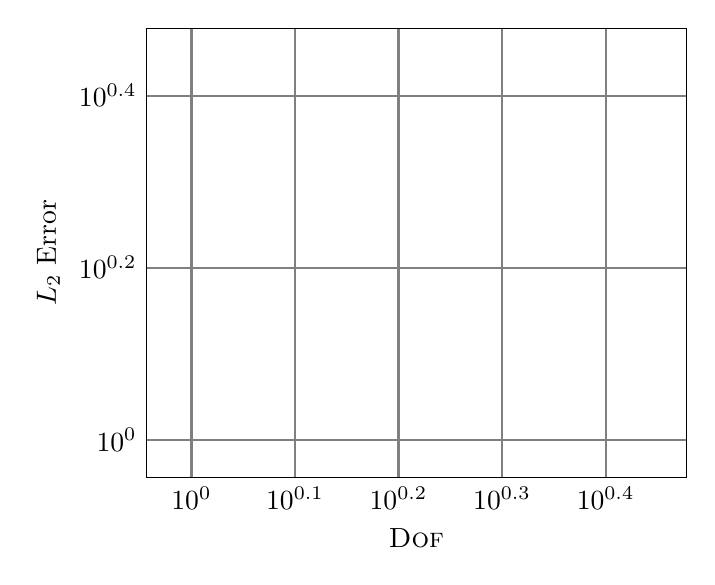
\begin{tikzpicture}
\begin{loglogaxis}[
    xlabel={\textsc{Dof}},
    ylabel={$L_2$ Error},
    grid=major,
]
    % see above for this macro:
    \plotcoords
\end{loglogaxis}
\end{tikzpicture}
\end{codeexample}

\begin{codeexample}[]
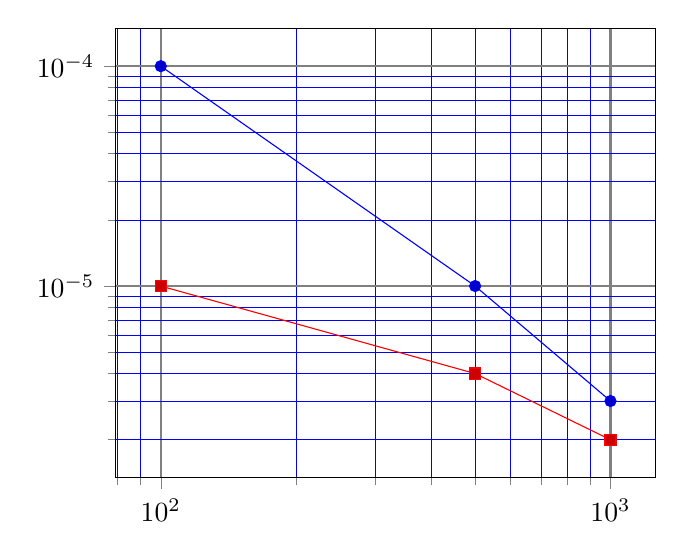
\begin{tikzpicture}
\begin{loglogaxis}[
    grid=both,
    tick align=outside,
    tickpos=left,
]
    \addplot coordinates {
        (100,1e-4) (500,1e-5) (1000,3e-6)
    };
    \addplot coordinates {
        (100,1e-5) (500,4e-6) (1000,2e-6)
    };
\end{loglogaxis}
\end{tikzpicture}
\end{codeexample}

    网格线会在刻度线处理之前绘制，因此刻度会绘制在网格线之上。你可以使用以下样式配置网格线的外观：
    %
\begin{codeexample}[code only]
\pgfplotsset{grid style={help lines}} % modifies the style `every axis grid'
\pgfplotsset{minor grid style={color=blue}} % modifies the style `every minor grid'
\pgfplotsset{major grid style={thick}} %modifies the style `every major grid'
\end{codeexample}
\end{pgfplotsxykeylist}


\section{自定义注释}
\label{sec:pgfplots:annotations}

通常，人们可能想向坐标轴添加自定义绘图元素或描述性文本。这些图形元素应该关联到某个逻辑坐标、网格点，或者只是放置到坐标轴中的某个位置。

在注释方面，\PGFPlots{} 提供以下方式的辅助：
%
\begin{enumerate}
    \item 你可以向坐标轴显式提供任何 \Tikz{} 指令，如 |\draw ... ;|。这里，|axis cs| 允许提供 \PGFPlots{} 的坐标。

        此外，|rel axis cs| 允许相对地放置 \Tikz{} 元素（如“坐标轴宽度的 $50\%$”）。\item \PGFPlots{} 可以使用其 |nodes near coords| 功能在每个坐标处自动生成节点。
    %\item \PGFPlots{} can automatically generate \Tikz{} labels for every coordinate (FIXME).
    \item \PGFPlots{} 允许你使用 |\addplot ... node[pos=|\meta{fraction}|] {};| 功能在图上放置节点。
\end{enumerate}
%
本节解释所有这些方法，除了 |nodes near coords| 功能（它在自己的小节中记录）。


\subsection{在图形元素中访问坐标轴坐标}
\label{sec:axis:coords}

\begin{coordinatesystem}{axis cs}
    \PGFPlots{} 提供了一个在坐标轴内部使用的新坐标系，即“坐标轴坐标系”，|axis cs|。

    请注意，每当在坐标轴中编写图形元素时，这个坐标系实际上就是默认坐标系。只有一个地方你真正需要显式提供这个坐标系：当你使用 |symbolic x coords| 时。

    因此，你可以将本文档仅作为参考；大多数标准用例可直接工作（自 |compat=1.11| 起）。

    它可用于在坐标轴坐标处绘制任何 \Tikz{} 图形。它的用法如下：
    %
\begin{codeexample}[code only]
\draw
       (axis cs:18943,2.873391e-05)
    |- (axis cs:47103,8.437499e-06);
\end{codeexample}

\begin{codeexample}[]
\tikzstyle{every pin}=[
    fill=white,
    draw=black,
    font=\footnotesize,
]
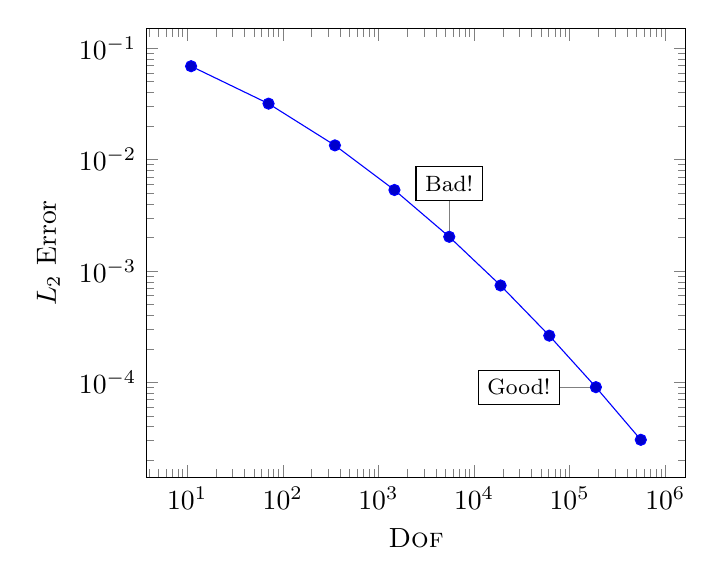
\begin{tikzpicture}
\begin{loglogaxis}[
    xlabel={\textsc{Dof}},
    ylabel={$L_2$ Error},
]
    \addplot coordinates {
        (11,     6.887e-02)
        (71,     3.177e-02)
        (351,    1.341e-02)
        (1471,   5.334e-03)
        (5503,   2.027e-03)
        (18943,  7.415e-04)
        (61183,  2.628e-04)
        (187903, 9.063e-05)
        (553983, 3.053e-05)
    };

    \node [coordinate,pin=above:{Bad!}]
        at (axis cs:5503,2.027e-03)   {};
    \node [coordinate,pin=left:{Good!}]
        at (axis cs:187903,9.063e-05) {};
    \end{loglogaxis}
\end{tikzpicture}
\end{codeexample}

    然而，由于 |axis cs| 是 \PGFPlots{} 的默认坐标系，你可以在坐标描述中简单地省略前缀 |axis cs:|。\footnote{自 \PGFPlots{} 1.11 版和 \verb|compat=1.11| 起。所有旧版本都显式需要该前缀；没有前缀的坐标会被放置在错误的位置。}
    %
\begin{codeexample}[]
\begin{tikzpicture}
\begin{loglogaxis}[
    xlabel=\textsc{Dof},
    ylabel=$L_2$ Error,
]
    \draw
            (1793,4.442e-05)
        |-  (4097,1.207e-05)
            node [near start,left]
                {$\frac{dy}{dx} = -1.58$};

    \addplot coordinates {
        (5,    8.312e-02)
        (17,   2.547e-02)
        (49,   7.407e-03)
        (129,  2.102e-03)
        (321,  5.874e-04)
        (769,  1.623e-04)
        (1793, 4.442e-05)
        (4097, 1.207e-05)
        (9217, 3.261e-06)
    };
\end{loglogaxis}
\end{tikzpicture}
\end{codeexample}

    |axis cs| 的效果是应用任何自定义变换（包括 |symbolic x coords|）、对数、数据缩放变换或 \PGFPlots{} 通常做的任何事情，并提供一个底层 \pgfname{} 坐标作为结果。

    如果你只需要这样一个向量的一个分量（比如 $y$ 分量），可以使用 |\pgfplotstransformcoordinatey| 命令；有关底层访问的详细信息，请参见 Section~\ref{sec:basic:coordinates}。

    |axis cs| 的结果始终是坐标轴内部的绝对位置。这尤其意味着\emph{相加}两个点会产生意外效果：表达式 |(0,0) ++ (1,0)| 不一定与 |(1,0)| 相同。这种意外效果的背景是，\PGFPlots{} 应用了一个\emph{平移的}线性变换，它移动原点以支持其高精度和高数据范围（参见 |disabledatascaling| 的文档）。

    为了表示\emph{相对}位置（或长度），你需要使用 |axis direction cs|。
\end{coordinatesystem}

\begin{coordinatesystem}{axis direction cs}
    虽然 |axis cs| 允许提供\emph{绝对位置}，但 |axis direction cs| 提供\emph{方向}。它允许通过坐标轴坐标来表示\emph{相对}位置，包括长度和尺寸。

    如 |axis cs| 文档中所述，通过 \tikzname{} 的 |++| 运算符相加两个坐标可能会产生意外效果。|++| 运算的正确方式是 |axis direction cs|：
    %
\begin{codeexample}[]
\begin{tikzpicture}
\begin{axis}
    \draw [red,-stealth]
        (1000,0)
        --  % = line-to
        ++ % = calculate a vector sum
        (axis direction cs:1000,0);

    \addplot [only marks,mark=*]
        coordinates { (1000,0) (2000,1) };
\end{axis}
\end{tikzpicture}
\end{codeexample}
    %
    \noindent 这里，红色箭头的目标是位置 |(2000,0)|，与预期一致。

    使用相对位置主要对线性坐标轴有用。将此命令应用于对数坐标轴可能仍然有效，但需要更加小心。

    一个用例是提供长度——例如为了支持 |circle| 或 |ellipse| 路径。在 \PGFPlots{} 中绘制椭圆的正确方式是通过两个 |(axis direction cs:|\meta{x,y}|)| 表达式来指定涉及的两个半径。一般来说，如果你使用底层宏 |\pgfpathellipse| 和 |\pgfplotspointaxisdirectionxy|，这是可行的。有关通过此方法绘制任意椭圆的两个示例，请参阅 |\pgfplotspointaxisdirectionxy| 的文档。

    由于在坐标轴内部绘制圆和椭圆是一个常见用例，\PGFPlots{} 会自动将其坐标系变换传达给 \tikzname：每当你写入 |\draw ellipse[|\declareandlabel{x radius}|=|\meta{x}|,|\declareandlabel{y radius}|=|\meta{y}|]| 时，参数 \meta{x} 和 \meta{y} 被视为 \PGFPlots{} 方向向量，并被交给 |axis direction cs|。因此，具有坐标轴平行半径的椭圆非常简单，并使用正常的 \tikzname{} 语法：
    %
\begin{codeexample}[]
% requires \pgfplotsset{compat=1.5.1} !
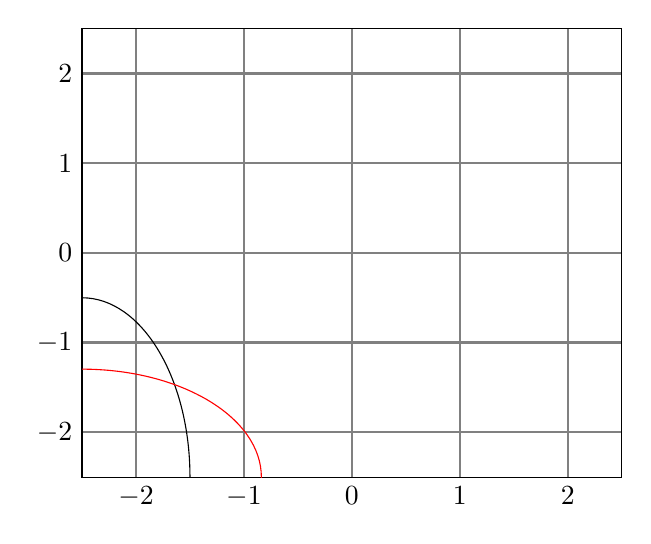
\begin{tikzpicture}
\begin{axis}[
    xmin=-2.5,   xmax=2.5,
    ymin=-2.5,   ymax=2.5,
    xtick={-2,-1,0,1,2},
    ytick={-2,-1,0,1,2},
    grid=major,
]
    % standard tikz syntax:
    \draw [black] (0,0) ellipse [
        x radius=1,
        y radius=2,
    ];
    \draw [red]   (0,0) ellipse [
        rotate=90,
        x radius=1,
        y radius=2,
    ];
    % see \pgfplotspointaxisdirectionxy
    % for arbitrary ellipses
\end{axis}
\end{tikzpicture}
\end{codeexample}
    %
    这里，两个椭圆像往常一样在 \tikzname 中指定。\PGFPlots{} 确保所有必要的变换都应用于这两个半径。请注意，\PGFPlots{} 通常对 $x$ 和 $y$ 有不同的坐标轴缩放。因此，旋转后的红色椭圆不适合坐标轴线；我们需要使用 |axis equal| 才能允许正确旋转的椭圆。


    \paragraph{注意：}

    这种对圆和椭圆的修改需要 |\pgfplotsset{compat=1.5.1}|。

    圆也是如此：在标准视图中，由于坐标轴缩放不同，半径为 \declareandlabel{radius}|=|$r$ 的圆会显示为椭圆。提供 |axis equal| 会得到真正的圆：
    %
\begin{codeexample}[]
% requires \pgfplotsset{compat=1.5.1} !
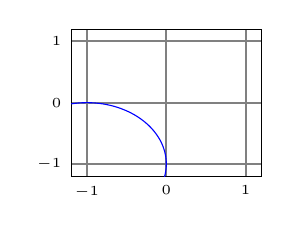
\begin{tikzpicture}
\begin{axis}[tiny,enlargelimits,
    xmin=-1,xmax=1,
    ymin=-1,ymax=1,
    xtick={-1,0,1},
    ytick={-1,0,1},
    grid=major,
]
    \draw [blue] (0,0) circle [radius=1];
\end{axis}
\end{tikzpicture}
\end{codeexample}
\begin{codeexample}[]
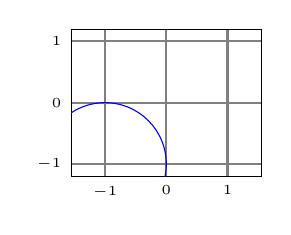
\begin{tikzpicture}
\begin{axis}[tiny,enlargelimits,
    axis equal,
    xmin=-1,xmax=1,
    ymin=-1,ymax=1,
    xtick={-1,0,1},
    ytick={-1,0,1},
    grid=major,
]
    \draw [blue] (0,0) circle [radius=1];
\end{axis}
\end{tikzpicture}
\end{codeexample}

    如果你需要在数学表达式内部访问 |axis direction cs|，可以使用附加数学函数 \declareandlabel{transformdirectionx}。它与 |axis direction cs| 作用相同，但仅在 $x$ 方向上。|transformdirectionx| 的结果是一个无量纲单位，可以相对于当前 \pgfname{} 的 $x$ 单位向量 $e_x$ 来解释（详情参见 |\pgfplotstransformdirectionx| 的文档）。还有数学命令 |transformdirectionx|、\declareandlabel{transformdirectiony}，以及（如果坐标轴是三维的）\declareandlabel{transformdirectionz}。它们中的每一个都定义 |\pgfmathresult| 以包含 |\pgfplotstransformdirectionx| 的结果（或其针对 $y$ 和 $z$ 的变体）。
\end{coordinatesystem}

\begin{coordinatesystem}{rel axis cs}
    “相对坐标轴坐标系”，|rel axis cs|，使用完整的坐标轴向量作为单位。这意味着 `$x=0$' 表示 $x$ 轴范围下端的点，`$x=1$' 表示 $x$ 轴范围上端的点（关于 |x dir=reverse| 见下文说明）。
    %
\pgfplotsexpensiveexample
\begin{codeexample}[]
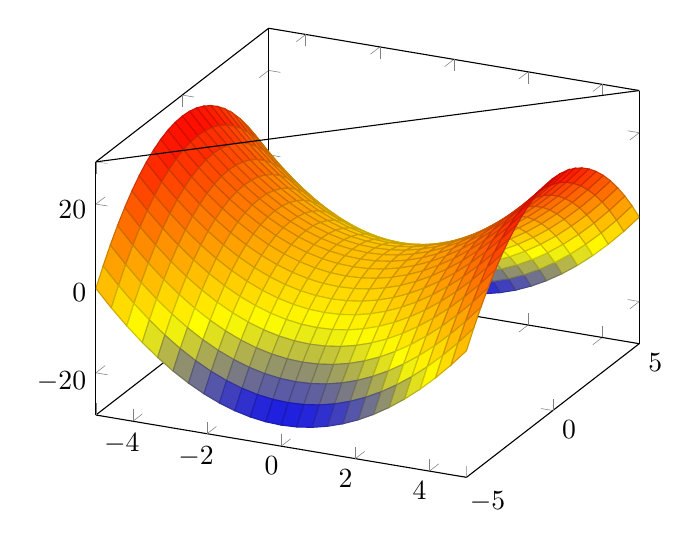
\begin{tikzpicture}
\begin{axis}
    \addplot3 [surf] {x^2 - y^2};
    \draw  (rel axis cs:0,0,1)
        -- (rel axis cs:1,1,1);
\end{axis}
\end{tikzpicture}
\end{codeexample}

\pgfplotsexpensiveexample
\begin{codeexample}[]
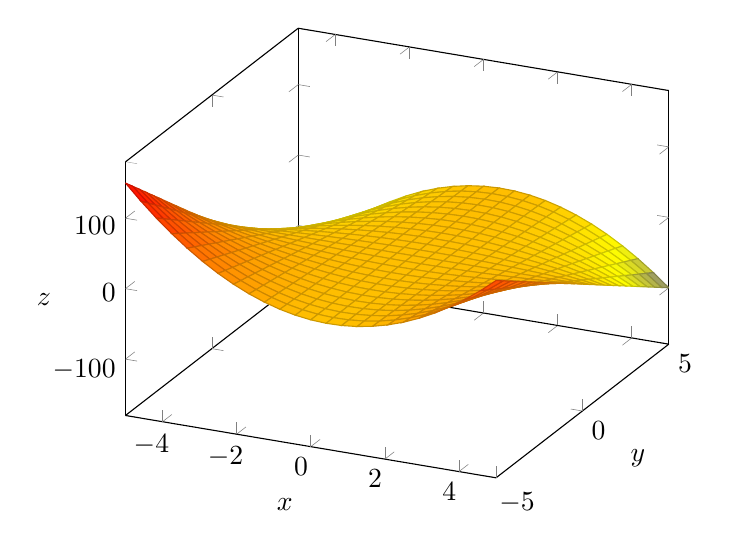
\begin{tikzpicture}
\begin{axis}[
    xlabel=$x$,
    ylabel=$y$,
    zlabel=$z$,
    every axis x label/.style={
        at={(rel axis cs:0.5,-0.15,-0.15)}},
    every axis y label/.style={
        at={(rel axis cs:1.15,0.5,-0.15)}},
    every axis z label/.style={
        at={(rel axis cs:-0.15,-0.15,0.5)}},
]
    \addplot3 [surf] {x*(1-x)*y};
\end{axis}
\end{tikzpicture}
\end{codeexample}

    由 |rel axis cs| 标识的点使用语法

        |(rel axis cs:|\meta{x}|,|\meta{y}|)| 或

        |(rel axis cs:|\meta{x}|,|\meta{y}|,|\meta{z}|)|

    \noindent 其中 \meta{x}、\meta{y} 和 \meta{z} 是坐标或常数数学表达式。第二种语法仅在三维坐标轴中可用。

    有一个特殊之处：如果你反转坐标轴（使用 |x dir=reverse|），由 |rel axis cs| 提供的点将\emph{不受}坐标轴反转的影响。这是为了即使在反转坐标轴时也能提供一致的放置。使用 |allow reversal of rel axis cs=false| 可禁用此功能。

    还有一个底层接口用于访问变换和坐标，参见第~\pageref{cha:pgfplots:lowlevel} 页的 Chapter~\ref{cha:pgfplots:lowlevel}。
\end{coordinatesystem}

\begin{predefinednode}{current plot begin}
    此坐标将为每个图定义，并可用作 \meta{trailing path commands} 或在图之后使用。它是当前图的第一个坐标。
\end{predefinednode}

\begin{predefinednode}{current plot end}
    此坐标将为每个图定义。它是当前图的最后一个坐标。
\end{predefinednode}

\begin{pgfplotskey}{allow reversal of rel axis cs=\mchoice{true,false} (initially true)}
    一个微调键，用于指定如何处理 |x dir=reverse| 与 |rel axis cs| 和 |ticklabel cs|。

    初始配置 |true| 表示使用 |rel axis cs| 和/或 |ticklabel cs| 放置的点在坐标轴内部将处于相同位置，即使其顺序已被反转。选项 |false| 将禁用对 |x dir=reverse| 的特殊处理。
\end{pgfplotskey}


\subsection{更改单个坐标的外观}
\label{sec:coordinate:style}

某些绘图处理器，尤其是 |scatter| 图的各种变体，支持修改单个标记的外观。为此，它们接受语法 |coordinate style|：\index{coordinate style}
%
\begin{codeexample}[]
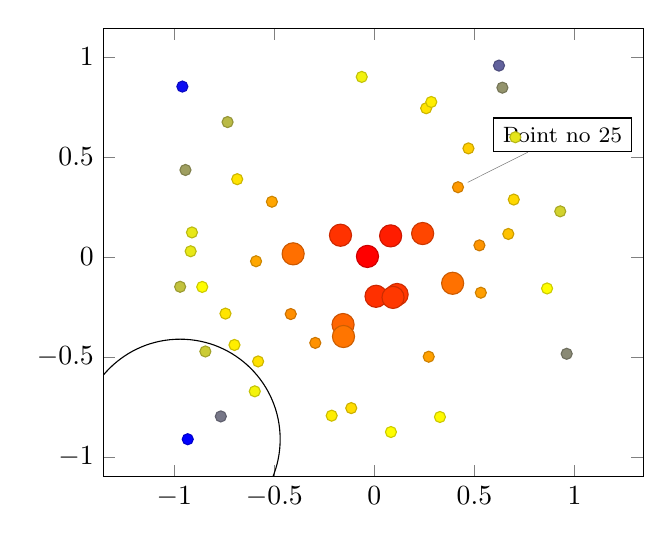
\begin{tikzpicture}
\begin{axis}[axis equal]
  \addplot[
    scatter,
    only marks,
    samples=50,
    point meta=100-sqrt(x^2+y^2),
    coordinate style/.condition=
        {sqrt(x^2+y^2) < 0.5}{scale=2},
    coordinate style/.condition={\coordindex == 25}{
      /pgfplots/scatter/@post marker code/.add code={
        \node [pin=45:Point no 25] {};
      }{},
    },
  ] (rand,rand);

  \draw (0,0) circle (0.5);
\end{axis}
\end{tikzpicture}
\end{codeexample}
%
上例是一个随机点散点图。第一个 |coordinate style| 确保落入半径为 $0.5$ 的圆内的所有点都绘制为两倍大小。第二个 |coordinate style| 对索引为 $25$ 的点应用特殊绘图指令：它附加一个 |pin|。

键 |coordinate style| 在第~\pageref{key:coordinatestyle} 页记录。


\subsection{在图的坐标上放置节点}
{
\tikzset{external/figure name/.add={}{nodes_}}

|\addplot| 命令不仅用于 \PGFPlots{}，它还可以携带附加的绘图指令，这些指令在图的路径完成后被交给 \Tikz{}。其中，这可用于在路径上添加更多节点。

\begin{key}{/tikz/pos=\marg{fraction}}
    如果 \meta{fraction} 在结尾分号之前使用，它标识最近完成的图的一部分：
    %
\pgfplotsexpensiveexample
\begin{codeexample}[]
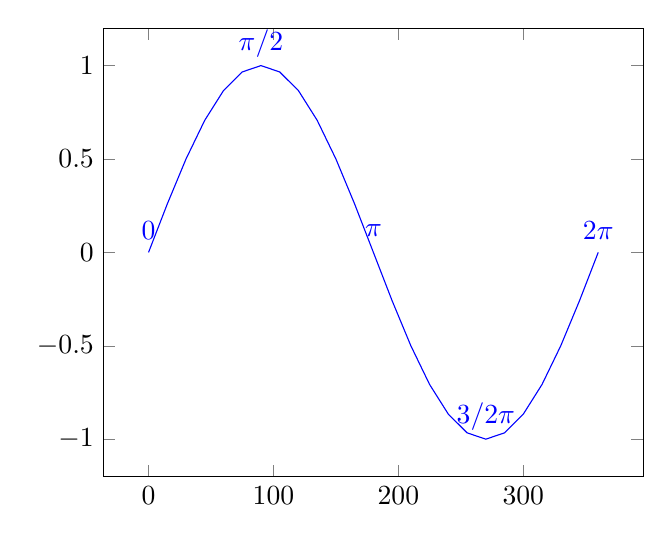
\begin{tikzpicture}
\begin{axis}
    \addplot [blue,domain=0:360] {sin(x)}
        [yshift=8pt]
            node [pos=0]    {$0$}
            node [pos=0.25] {$\pi/2$}
            node [pos=0.5]  {$\pi$}
            node [pos=0.75] {$3/2\pi$}
            node [pos=1]    {$2\pi$}
    ;
\end{axis}
\end{tikzpicture}
\end{codeexample}
%
    \noindent 这里，|[yshift=8pt]| 告诉 \Tikz{} 将所有后续节点向上偏移。|node[pos=0] {$0$}| 指令告诉 \Tikz{} 在最近完成的图的 $0\%$ 处添加一个文本节点。相对位置 $0\%$（|pos=0|）指 \PGFPlots{} 看到的第一个坐标，$100\%$（|pos=1|）指最后一个坐标。$0$ 到 $1$ 之间的任何值都在其间插值。请注意，所有这些节点都属于图的可视化（以分号结束）。因此，所有这些节点都继承相同的图形设置（如颜色选择）。

    图上的位置由 \PGFPlots{} 使用\emph{逻辑}坐标计算。这意味着：它在曲线投影到屏幕坐标之前计算曲线的总长度，并标识所需位置。\footnote{这可能是一个耗时的过程。如果你有很多这样的图，请考虑使用 external 库。}之后，它将最终位置投影到屏幕坐标。因此，该位置标识图上的一个位置，即使在旋转的三维坐标轴情况下也始终相同。\PGFPlots{} 将在相邻坐标之间线性插值该比例。

    \meta{fraction} 的有效选择是范围 $[0,1]$ 内的任何数字。

    请注意，|pos| 的确切含义取决于当前绘图处理器：对于大多数绘图处理器，它默认为线性插值（如上例）。对于 |only marks|、|scatter|、|ybar|、|xbar|、|ybar interval| 和 |xbar interval|，它会吸附到遇到的最近坐标。在此上下文中，“吸附到最近”表示 |pos=|$p$ 指向索引为 $i = \text{round}(p \cdot N)$ 的坐标，其中 $N$ 是点的总数：
    %
\begin{codeexample}[]
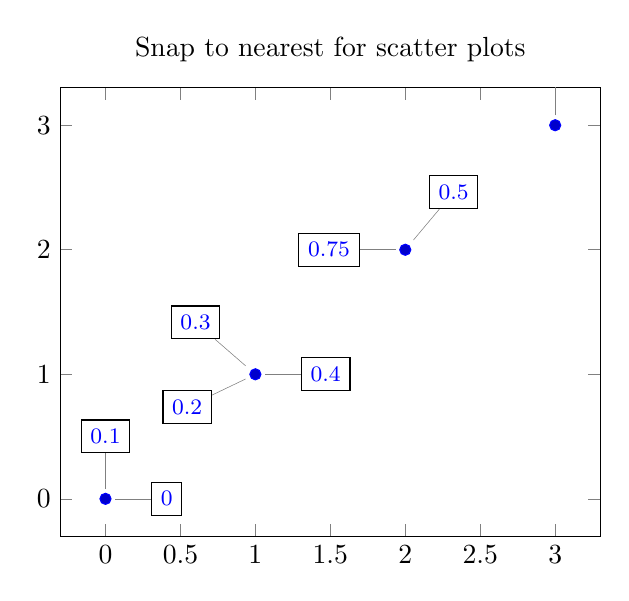
\begin{tikzpicture}
\begin{axis}[title=Snap to nearest for scatter plots]
    \addplot+ [only marks]
        coordinates { (0,0) (1,1) (2,2) (3,3) }
            node [pos=0,   pin=0  :0   ] {}
            node [pos=0.1, pin=90 :0.1 ] {}
            node [pos=0.2, pin=200:0.2 ] {}
            node [pos=0.3, pin=135:0.3 ] {}
            node [pos=0.4, pin=0  :0.4 ] {}
            node [pos=0.5, pin=60 :0.5 ] {}
            node [pos=0.75,pin=180:0.75] {}
            node [pos=1,   pin=90 :1   ] {}
    ;
\end{axis}
\end{tikzpicture}
\end{codeexample}
    %
    \noindent 上例表明 |pos=|$p$ 映射到四个可用坐标之一，即索引最接近 $p\cdot N$ 的那个。请注意，在这种情况下，坐标之间的距离无关紧要——只有坐标索引算数。

    请注意，如果 $x$ 和 $y$ 坐标轴在不同的缩放比例上运行，\PGFPlots{} 使用\emph{逻辑}坐标计算目标位置这一事实可能会产生意外效果。例如，假设 $x$ 总是在 $10^3$ 量级，而 $y$ 在 $10^{-3}$ 量级。在这种情况下，$y$ 坐标对曲线长度没有显著贡献——尽管重新缩放的坐标轴清楚地显示了“显著的” $y$ 动态。考虑将 |axis equal| 与 |pos| 一起使用以产生可比的效果。
\end{key}

\begin{key}{/tikz/sloped (initially false)}
    为以 |pos| 标识的节点提供 \Tikz{} 键 |sloped| 会使其旋转，以适应图的梯度。
    %
\pgfplotsexpensiveexample
\begin{codeexample}[]
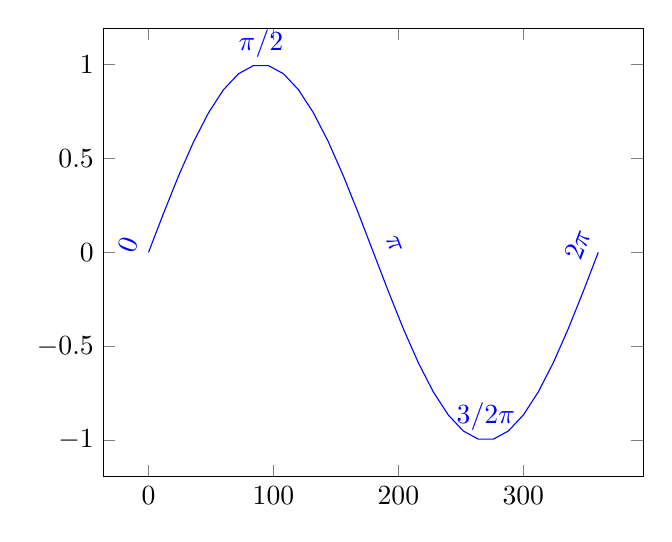
\begin{tikzpicture}
\begin{axis}
    \addplot [blue,domain=0:360,samples=31] {sin(x)}
        [every node/.style={yshift=8pt},sloped]
            node [pos=0]    {$0$}
            node [pos=0.25] {$\pi/2$}
            node [pos=0.5]  {$\pi$}
            node [pos=0.75] {$3/2\pi$}
            node [pos=1]    {$2\pi$}
    ;
\end{axis}
\end{tikzpicture}
\end{codeexample}
    %
    请注意，应用 |sloped| 和偏移变换的顺序很重要：如果先应用偏移（就像没有 |every node/.style| 结构时的情况那样），偏移不会考虑旋转。如果先应用 |sloped|，则任何后续偏移都将在\emph{旋转后}的坐标中应用。因此，情况 |every node/.style={yshift=8pt}| 会将每个节点沿其法线向量方向偏移 |8pt|。

    |sloped| 变换基于两个点之间的梯度（与 |pos| 相邻的两个点）。因此，它继承了任何采样弱点。为了看到这一点，考虑上面示例使用不同的采样数量：
    %
\pgfplotsexpensiveexample
\begin{codeexample}[]
% same as above with different number of samples
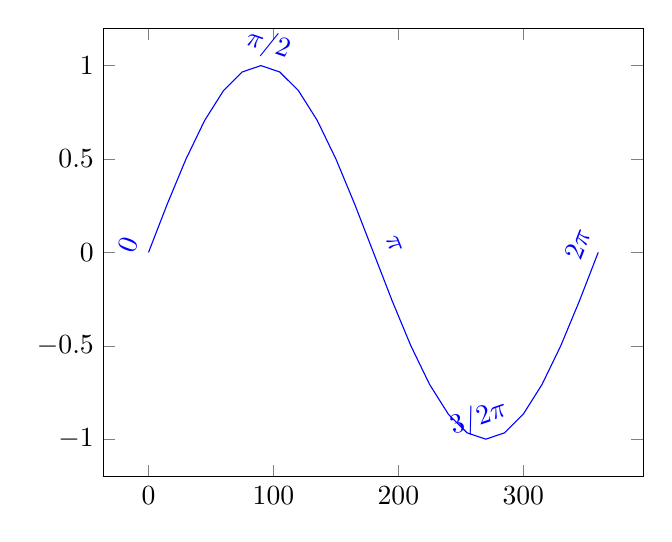
\begin{tikzpicture}
\begin{axis}
    \addplot [blue,domain=0:360,samples=25] {sin(x)}
        [every node/.style={yshift=8pt},sloped]
            node [pos=0]    {$0$}
            node [pos=0.25] {$\pi/2$}
            node [pos=0.5]  {$\pi$}
            node [pos=0.75] {$3/2\pi$}
            node [pos=1]    {$2\pi$}
    ;
\end{axis}
\end{tikzpicture}
\end{codeexample}
    %
    \noindent 这里，由于采样，两个端点具有较小的斜率。虽然这不会严重影响图的质量，但它对变换矩阵有巨大影响。在使用 |sloped| 时请记住这一点（也许添加一个额外的 |rotate| 参数甚至会有帮助）。
\end{key}

\begin{key}{/tikz/allow upside down=\mchoice{true,false} (initially false)}
    如果启用了 |/tikz/sloped| 并且有一些复杂的线图，变换可能导致节点被倒置绘制。默认配置 |allow upside down=false| 会切换旋转矩阵，而 |allow upside down| 允许这种情况。
\end{key}

\begin{key}{/tikz/pos segment=\marg{segment index} (initially empty)}
    偶尔，一个图由多个段组成（如由 |empty line=jump| 或 |contour prepared| 生成的那些）。各个段通常具有不同的长度，因此在其中一个段上标识位置很繁琐。

    如果 |pos segment=|\meta{segment index} 非空，则键 |pos=|\meta{fraction} 相对于所提供的段而非整个图来解释。参数 \meta{segment index} 是一个整数，其中 $0$ 表示第一个段。
    %
\begin{codeexample}[]
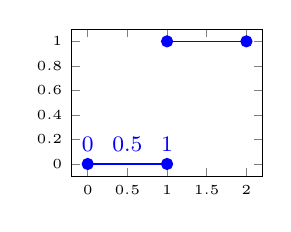
\begin{tikzpicture}
\begin{axis}[tiny]
    \addplot coordinates {
        (0,0) (1,0)

        (1,1) (2,1)
    }
        [pos segment=0,yshift=7pt,font=\footnotesize]
            node [pos=0] {0}
            node [pos=0.5] {0.5}
            node [pos=1] {1};
\end{axis}
\end{tikzpicture}
\end{codeexample}
    %
    这里，图有两个段。然而，所有三个注释节点都使用 |pos segment=0| 放置。

\pgfplotsexpensiveexample
\begin{codeexample}[]
\begin{tikzpicture}
\begin{axis}
    \addplot3 [contour lua,domain=0:1] {x*y}
        [sloped,
         allow upside down,
         pos segment=2,
         every node/.style={yshift=7pt},
        ]
            node [pos=0]   {0}
            node [pos=0.5] {0.5}
            node [pos=1]   {1}
        ;
\end{axis}
\end{tikzpicture}
\end{codeexample}
    %
    这个图有四个段（由绘图处理器自动生成）。注释节点放置在第三个段上，其中 |sloped| 使它们旋转，|allow upside down| 改善 `$0$' 的渲染，而 |every node/.style| 沿法线向量方向安装一个偏移（详情参见 |sloped| 的文档）。
\end{key}

偶尔，人们想使用 |pos| 放置一个节点，\emph{并且}想在节点内部排版该点的坐标。这可以使用 |\pgfplotspointplotattime| 来完成：

\begin{commandlist}{\pgfplotspointplotattime,\pgfplotspointplotattime\marg{fraction}}
    此命令是 |pos=|\marg{fraction} 实现的一部分：它将 \pgfname{} 的当前点定义为当前图的 \meta{fraction} 处。如果没有花括号中的参数，|\pgfplotspointplotattime| 将采用 |pos| 键的当前参数。

    因此，该命令计算基本 \pgfname{} 坐标——但它还将结果点的\emph{逻辑}坐标返回到以下键中：

    \begin{pgfplotsxykeylist}{/data point/\x}
        在 |\pgfplotspointplotattime| 返回后，这些宏包含结果点的 $x$、$y$ 和 $z$ 坐标。例如，可以通过 |\pgfkeysvalueof{/data point/x}| 来使用它们。
        %
\begin{codeexample}[]
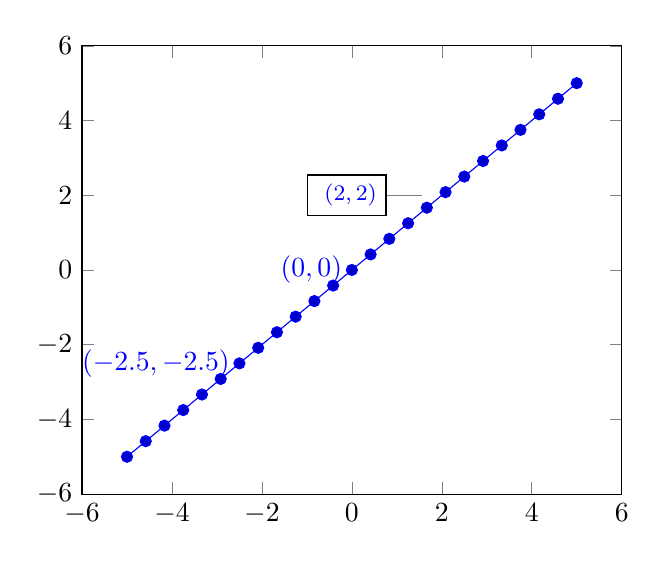
\begin{tikzpicture}
\begin{axis}
    \addplot {x}
      [left,/pgf/number format/relative=0]
        node [pos=0.5] {
            \pgfplotspointplotattime
            $(\pgfmathprintnumber
                  {\pgfkeysvalueof{/data point/x}},
              \pgfmathprintnumber
                  {\pgfkeysvalueof{/data point/y}})$
        }
        node [pos=0.25] {
            \pgfplotspointplotattime
            $(\pgfmathprintnumber
                  {\pgfkeysvalueof{/data point/x}},
              \pgfmathprintnumber
                  {\pgfkeysvalueof{/data point/y}})$
        }
        node [pos=0.7,pin=180:{
            \pgfplotspointplotattime{0.7}
            $(\pgfmathprintnumber
                  {\pgfkeysvalueof{/data point/x}},
              \pgfmathprintnumber
                  {\pgfkeysvalueof{/data point/y}})$
        }] {}
    ;
\end{axis}
\end{tikzpicture}
\end{codeexample}

        在上面的示例中，使用不同的 |pos=| 参数放置了三个节点。在相关节点的主体内部调用 |\pgfplotspointplotattime| 会检查 |pos| 是否已有值并使用该值。第三个节点在 |pin| 内部显示坐标。由于 \tikzname 的内部机制，|pin| 对其外层 |node| 的 |pos=0.7| 参数一无所知，因此我们需要为 |\pgfplotspointplotattime{0.7}| 复制 `|0.7|' 参数。|/pgf/number format/relative=0| 样式使数字打印机相对于 $10^0$ 取整（与没有此样式的同一示例比较）。

        如果你使用 |symbolic x coords|（或任何其他产生非数字结果的 |x coord inv tafo|），存储在 |/data point/x| 中的输出将是符号表达式：
        %
\begin{codeexample}[]
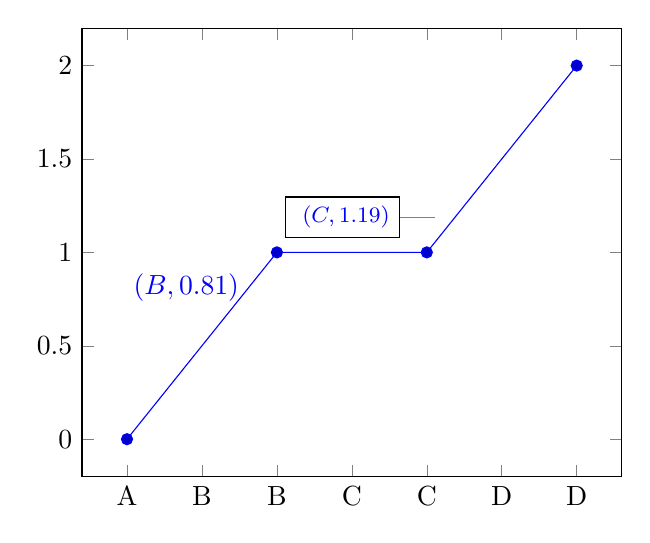
\begin{tikzpicture}
\begin{axis}[symbolic x coords={A,B,C,D}]
    \addplot coordinates {(A,0) (B,1) (C,1) (D,2)}
        [left]
            node [pos=0.3] {
                \pgfplotspointplotattime
                $(\pgfkeysvalueof{/data point/x},
                  \pgfmathprintnumber
                    {\pgfkeysvalueof{/data point/y}})$
            }
            node [pos=0.7,pin=180:{
                \pgfplotspointplotattime{0.7}
                $(\pgfkeysvalueof{/data point/x},
                  \pgfmathprintnumber
                    {\pgfkeysvalueof{/data point/y}})$
            }] {}
    ;
\end{axis}
\end{tikzpicture}
\end{codeexample}
        %
        \noindent 在那种特定情况下，你必须避免使用 |\pgfmathprintnumber|，因为该参数\emph{不是}数字。请注意，|symbolic x coords| 不能像你预期的那样返回 $A$ 和 $B$ 之间的分数。然而，该点仍将放置在分数位置（除非你使用 |scatter| 或 |bar| 图）。

        对于有很多点的图，|pos| 功能的坐标计算在计算上很昂贵。为了减少时间，\PGFPlots{} 会缓存计算出的值：使用相同参数多次调用命令 |\pgfplotspointplotattime| 将重用计算出的值。
    \end{pgfplotsxykeylist}
\end{commandlist}

}


\subsection{在图之上放置装饰}

{
\tikzset{external/figure name/.add={}{decorations_}}

\tikzname{} 附带强大的 \declareandlabel{decorations} 库（或者更准确地说：一组库）。装饰允许通过花哨的附加图形来替换或扩展现有路径。\tikzname{} 装饰功能的介绍超出了本手册的范围，感兴趣的读者应阅读~\cite{tikz} 中的相关章节。

本节展示如何使用装饰来增强 \PGFPlots{} 中的图。假设你有一些图形，想为其添加“方向指针”：
%
\begin{codeexample}[]
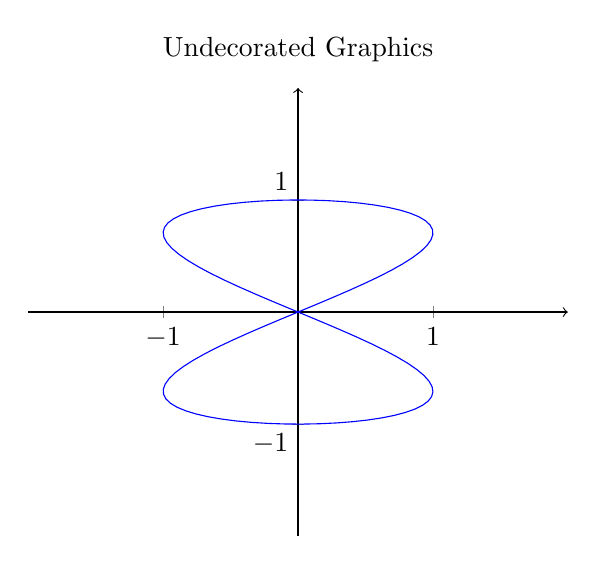
\begin{tikzpicture}[]
% An undecorated graphics with a lot of
% pretty-printing styles:
\begin{axis}[
    axis lines=middle,
    title=Undecorated Graphics,
    xmin=-2, xmax=2, ymin=-2, ymax=2,
    xtick={-1,1}, ytick={-1,1},
    % this disables the standard
    % tick label *text* (but not the line)
    yticklabel=\ ,
    extra description/.code={
        % this generates custom y labels to implement
        % individual styles for every tick:
        \node [below left] at (axis cs:0,-1) {$-1$};
        \node [above left] at (axis cs:0,1) {$1$};
    },
    axis line style={->},
]
    \addplot [blue,samples=100,domain=0:2*pi]
        ({sin(deg(2*x))}, {sin(deg(x))});
\end{axis}
\end{tikzpicture}
\end{codeexample}
%
\noindent 我们的目标是添加简短指针以指示参数化的方向。

解决方案是使用 |\usetikzlibrary{decorations.markings}| 并在 |\addplot| 内部使用一个装饰：
%
% \usetikzlibrary{decorations.markings}
\begin{codeexample}[]
% requires \usetikzlibrary{decorations.markings}
\begin{tikzpicture}[]
% Same as in previous example, but with decorations:
\begin{axis}[
    axis lines=middle,
    title=Decorated Graphics,
    xmin=-2, xmax=2, ymin=-2, ymax=2,
    xtick={-1,1}, ytick={-1,1},
    % this disables the standard
    % tick label *text* (but not the line)
    yticklabel=\ ,
    extra description/.code={
        % this generates custom y labels to implement
        % individual styles for every tick:
        \node [below left] at (axis cs:0,-1) {$-1$};
        \node [above left] at (axis cs:0,1) {$1$};
    },
    axis line style={->},
]
    \addplot[blue,samples=100,domain=0:2*pi,
      postaction={decorate},% ------
      decoration={markings, % ------
         mark=at position 0.25 with {\arrow{stealth}},
         mark=at position 0.5  with {\arrow{stealth}},
         mark=at position 0.75 with {\arrow{stealth}}}
    ] ({sin(deg(2*x))}, {sin(deg(x))});
\end{axis}
\end{tikzpicture}
\end{codeexample}
%
\noindent 唯一的更改在 |\addplot| 的选项列表中：它包含一个 \declareandlabel{postaction}|={|\declareandlabel{decorate}|}|，用于激活装饰（不替换原始路径），以及一些 \declareandlabel{decoration} 规范，其中包含如何装饰路径的详细信息。

|decorations| 库的详细讨论超出了本手册的范围（详情参见~\cite{tikz}），但要点是将所需的装饰添加到 |\addplot| 及其选项列表中。

}
